\documentclass[11pt,a4paper]{article}

% --- Πακέτα Γλώσσας & Γραμματοσειρών (Συμβατά με pdfLaTeX & XeLaTeX) ---
\usepackage[utf8]{inputenc}
\usepackage[LGR,T1]{fontenc}
\usepackage[greek,english]{babel}
\usepackage{alphabeta}

% --- Μορφοποίηση Σελίδας & Μαθηματικών ---
\usepackage[margin=2.2cm]{geometry}
\usepackage{amsmath,amssymb}
\usepackage{booktabs}
\usepackage{multirow}
\usepackage{float}
\usepackage{graphicx}
\usepackage{caption}
\usepackage{subcaption}
\usepackage{xcolor}
\usepackage{hyperref}
\setlength{\emergencystretch}{3em}

% --- Πακέτο Σχεδίασης Γραφημάτων ---
\usepackage{pgfplots}
\pgfplotsset{compat=1.18}

% --- Πακέτο Μορφοποίησης Κώδικα C/C++ ---
\usepackage{listings}

\definecolor{codebg}{rgb}{0.96,0.97,0.98}
\definecolor{codegreen}{rgb}{0.15,0.5,0.2}
\definecolor{codegray}{rgb}{0.45,0.45,0.45}
\definecolor{codeblue}{rgb}{0.1,0.3,0.7}

\lstdefinestyle{cstyle}{
    backgroundcolor=\color{codebg},
    commentstyle=\color{codegreen}\itshape,
    keywordstyle=\color{codeblue}\bfseries,
    numberstyle=\tiny\color{codegray},
    stringstyle=\color{purple},
    basicstyle=\ttfamily\footnotesize,
    breakatwhitespace=false,
    breaklines=true,
    captionpos=b,
    keepspaces=true,
    numbers=left,
    numbersep=6pt,
    showspaces=false,
    showstringspaces=false,
    showtabs=false,
    tabsize=4,
    frame=single,
    rulecolor=\color{black!20},
    language=C++
}
\lstset{style=cstyle}

% Λατινικό κείμενο μέσα σε ελληνικές προτάσεις
\newcommand{\en}[1]{\textlatin{#1}}

% --- Πληροφορίες Τίτλου ---
\title{
    \textbf{Εθνικό Μετσόβιο Πολυτεχνείο}\\
    \large Σχολή Ηλεκτρολόγων Μηχανικών και Μηχανικών Υπολογιστών\\
    \vspace{0.3cm}
    \textbf{Σχεδίαση Ενσωματωμένων Συστημάτων}\\
    \vspace{0.2cm}
    \Large 2η Εργαστηριακή Αναφορά: Βελτιστοποίηση Δυναμικών Δομών Δεδομένων (\en{DDTR}) και Δυναμική Διαχείριση Μνήμης (\en{DMM}) του Αλγορίθμου \en{NMS} στην Πλακέτα \en{AUP-ZU3}
}
\author{ΜΕΤΣΗΣ ΑΧΙΛΛΕΑΣ-ΟΔΥΣΣΕΑΣ -- Α.Μ.: 03117403 , ΙΑΣΩΝ ΖΑΚΥΝΘΙΝΟΣ -- 03123408}
\date{Νοέμβριος 2026}

\begin{document}

\maketitle

\hrule
\vspace{0.4cm}

\begin{abstract}
Ο αλγόριθμος \en{Non-Maximum Suppression (NMS)} είναι το τελευταίο στάδιο του ανιχνευτή αντικειμένων \en{YOLOv5}: από τα υποψήφια πλαίσια (\en{candidate boxes}) κάθε κλάσης κρατά εκείνο με τη μεγαλύτερη βεβαιότητα (\en{confidence}) και απορρίπτει όσα επικαλύπτονται μαζί του με \en{IoU} $> 0.45$. Η υλοποίηση της βιβλιοθήκης \en{tensorrtx} (\en{\texttt{postprocess.cpp}}) αποθηκεύει τα πλαίσια κάθε κλάσης σε \en{\texttt{std::vector<Detection>}} και αφαιρεί τα απορριφθέντα με \en{\texttt{erase}}. Στην άσκηση αυτή εφαρμόζουμε τη μεθοδολογία \en{DDTR} (αντικατάσταση της δομής με 9 δομές της βιβλιοθήκης \en{DDTR}) και \en{DMM} (4 δικοί μας \en{allocators} πάνω από \en{\texttt{mmap}}) και μετράμε στην πλακέτα \en{AUP-ZU3} τον χρόνο εκτέλεσης, το \en{memory footprint} και τα \en{misses} της τελευταίας στάθμης \en{cache}, για όλες τις 91 εκδοχές της εφαρμογής, στα δεδομένα \en{\texttt{detrac\_y5s\_640.bin}} με \en{confidence threshold} $0.05$.

Τα ερωτήματα της άσκησης που απαντώνται στην παρούσα αναφορά είναι:
\begin{enumerate}
    \item \textbf{Αρχική έκδοση:} Χρόνος εκτέλεσης και \en{memory footprint} της \en{\texttt{nms()}} της \en{tensorrtx} (\en{baseline}).
    \item \textbf{Βελτιστοποίηση δομών δεδομένων (\en{DDTR}):} Μεταφορά της \en{\texttt{nms()}} στη βιβλιοθήκη \en{DDTR}, μετρήσεις για τις 9 δομές και \en{Pareto plot} \en{memory footprint} -- χρόνου εκτέλεσης.
    \item \textbf{\en{Allocators} (\en{DMM}):} Υλοποίηση \en{arena}, \en{first fit} και \en{best fit allocator} (ο \en{worst fit} δόθηκε έτοιμος), μετρητές \en{\texttt{ALLOC\_STATS}} και \en{Pareto plot} για όλους τους συνδυασμούς δομής -- \en{allocator}.
    \item \textbf{\en{Flag} αντί για \en{erase}:} Εκδοχή της \en{\texttt{nms()}} που σημαδεύει τα απορριφθέντα πλαίσια σε ένα \en{vector} από \en{flags} αντί να τα αφαιρεί, και επανάληψη όλων των μετρήσεων.
\end{enumerate}

\vspace{0.3cm}
\hrule
\vspace{0.5cm}
\end{abstract}

% =============================================================================
\section{Πλατφόρμα και Μεθοδολογία Μετρήσεων}
% =============================================================================
\subsection{Η πλακέτα \en{AUP-ZU3}}
Η \en{AUP-ZU3} βασίζεται στο \en{SoC Zynq UltraScale+ ZU3EG} της \en{AMD/Xilinx}. Το λογισμικό τρέχει στον τετραπύρηνο \en{ARM Cortex-A53} (\en{in-order}, 64-\en{bit}) του \en{SoC}, με ιδιωτικές \en{L1} κρυφές μνήμες εντολών και δεδομένων ανά πυρήνα και κοινή \en{L2}, η οποία είναι και η τελευταία στάθμη \en{cache} (\en{LLC}). Η πλακέτα εκκινεί από την κάρτα \en{microSD} την εικόνα \en{PYNQ 3.1} (\en{Ubuntu 22.04}, \en{Linux 6.6.10}), και όλα τα εκτελέσιμα μεταγλωττίστηκαν πάνω στην πλακέτα με \en{g++ 11.2.0} (\en{\texttt{-O3 -std=c++17}}, μέσω του \en{\texttt{build.sh}}). Ο μετρητής \en{\texttt{cycles}} του \en{\texttt{perf}} έδειξε συχνότητα λειτουργίας $\approx 1.1$ \en{GHz} κατά τις μετρήσεις.

Ο κώδικας μεταφέρθηκε στην πλακέτα ως ένα αρχείο \en{\texttt{.tar.gz}} μέσω της \en{FAT} κατάτμησης της κάρτας \en{SD} (προσαρτημένη στο \en{\texttt{/boot}}) και αποσυμπιέστηκε στο \en{\texttt{/home/xilinx}}. Η επικοινωνία έγινε μέσω της σειριακής κονσόλας \en{UART} (115200 \en{baud}).

\subsection{Μέτρηση χρόνου εκτέλεσης}
Το \en{\texttt{main.cpp}} φορτώνει όλα τα \en{frames} του αρχείου εισόδου και μετρά με \en{\texttt{std::chrono::steady\_clock}} τον συνολικό χρόνο ενός περάσματος της \en{\texttt{nms()}} πάνω σε όλα τα \en{frames} (τυπώνει μια γραμμή \en{\texttt{ms=}} ανά πέρασμα). Για κάθε εκδοχή εκτελέσαμε το πρόγραμμα \textbf{3 φορές με \en{\texttt{runs=20}}}: για κάθε εκτέλεση υπολογίζεται ο μέσος όρος των 20 περασμάτων, και στους πίνακες δίνεται ο μέσος όρος και η (δειγματική) διακύμανση (\en{variance}) των 3 μέσων όρων. Η μέγιστη τυπική απόκλιση των 3 επαναλήψεων ήταν 0.6\% της μέσης τιμής, άρα οι μετρήσεις είναι πολύ σταθερές.

\subsection{Μέτρηση \en{LLC misses} με το \en{perf}}
Ο \en{Cortex-A53} δεν υποστηρίζει τα γενικά \en{events} \en{\texttt{LLC-load-misses}} και \en{\texttt{LLC-store-misses}} (το \en{\texttt{test\_perf.sh}} τα αναφέρει ως \en{\texttt{<not supported>}}). Επειδή η \en{L2} είναι η τελευταία στάθμη \en{cache}, μετρήσαμε το \en{event} \en{\texttt{l2d\_cache\_refill}}, που μετρά τα \en{refills} της \en{L2} από την κύρια μνήμη (φορτώσεις και εγγραφές μαζί, δεν διαχωρίζονται). Για κάθε εκδοχή:
\begin{itemize}
    \item \en{\texttt{perf stat -r 20 -e l2d\_cache\_refill ./exec input=... runs=1}}: ένα πέρασμα της \en{\texttt{nms()}} μαζί με τη φόρτωση των δεδομένων,
    \item το ίδιο με \en{\texttt{runs=0}}: μόνο η φόρτωση των δεδομένων και τα υπόλοιπα μέρη του προγράμματος.
\end{itemize}
Η διαφορά των δύο (\en{$\Delta$L2 refills}) αντιστοιχεί στην ίδια την \en{\texttt{nms()}} και είναι αυτή που δίνουμε στους πίνακες.

\subsection{Μέτρηση \en{memory footprint}}
Σύμφωνα με την εκφώνηση, το \en{Massif} εκτελέστηκε στο \en{PC}: σε \en{container Ubuntu 22.04 arm64}, δηλαδή ίδια αρχιτεκτονική και ίδια \en{glibc} με την πλακέτα, ώστε τα \en{bytes} του \en{heap} να είναι τα ίδια. Χρησιμοποιήθηκε η εντολή
\en{\texttt{valgrind --tool=massif --threshold=0 --peak-inaccuracy=0}}
και στο \en{snapshot (peak)} του \en{\texttt{ms\_print}} αθροίστηκαν οι κλάδοι του δέντρου που περνούν από την \en{\texttt{nms()}}. Το υπόλοιπο \en{heap} (το \en{\texttt{res.reserve(4096)}} της \en{\texttt{main}}, ο \en{emergency pool} της \en{libstdc++}, ο πίνακας δεικτών των \en{frames}) δεν αλλάζει από εκδοχή σε εκδοχή και δεν προσμετράται. Για τους δικούς μας \en{allocators}, που παίρνουν τη μνήμη τους με \en{\texttt{mmap}} (την οποία το \en{Massif} δεν βλέπει), το \en{footprint} δίνεται από τους μετρητές \en{\texttt{-DALLOC\_STATS}} (Ενότητα~\ref{sec:q3}).

Η ορθότητα κάθε εκδοχής ελέγχθηκε με \en{\texttt{-DVALIDATE}}: το εκτελέσιμο τρέχει και την αρχική \en{\texttt{nms()}} και συγκρίνει τα αποτελέσματα \en{frame} προς \en{frame}. Και οι 90 εκδοχές (9 δομές $\times$ 5 \en{allocators} $\times$ \{\en{erase}, \en{flag}\}) τύπωσαν \en{\texttt{validate: OK}}.

% =============================================================================
\section{Ζητούμενο 1: Αρχική Έκδοση της \en{NMS}}
% =============================================================================
Το εκτελέσιμο \en{\texttt{bin/nms-orig}} (\en{\texttt{./build.sh orig}}) χρησιμοποιεί την αρχική \en{\texttt{nms()}} της \en{tensorrtx}, με \en{\texttt{std::map<float, std::vector<Detection>>}} για την ομαδοποίηση ανά κλάση, \en{\texttt{std::sort}} και \en{\texttt{erase}} των απορριφθέντων πλαισίων. Τα αποτελέσματα δίνονται στους Πίνακες~\ref{tab:q1_time} και~\ref{tab:q1_mem}.

\begin{table}[H]
\centering
\caption{Execution time and LLC refills of the original \texttt{nms()} on the AUP-ZU3 (3 executions $\times$ 20 runs).}
\label{tab:q1_time}
\begin{tabular}{@{}lrrrrrr@{}}
\toprule
Version & Exec.~1 (ms) & Exec.~2 (ms) & Exec.~3 (ms) & Mean (ms) & Variance (ms$^2$) & $\Delta$L2 refills \\
\midrule
Original (\texttt{nms-orig}) & 347.5298 & 347.6427 & 347.4459 & 347.54 & 0.0098 & 185{,}186 \\
\bottomrule
\end{tabular}
\end{table}

\begin{table}[H]
\centering
\caption{Heap at the peak snapshot of Massif for the original version.}
\label{tab:q1_mem}
\begin{tabular}{@{}lrc@{}}
\toprule
Allocation site & Bytes & Part of \texttt{nms()} \\
\midrule
\texttt{main}: \texttt{res.reserve(4096)} ($4096 \times 152$ B) & 622{,}592 & no \\
\texttt{nms} $\rightarrow$ \texttt{vector<Detection>::\_M\_realloc\_insert} & 295{,}488 & \textbf{yes} \\
libstdc++ start-up (emergency exception pool) & 72{,}704 & no \\
\texttt{load()}: vector of frame pointers & 2{,}048 & no \\
\texttt{nms} $\rightarrow$ \texttt{std::map} nodes & 448 & \textbf{yes} \\
\midrule
\textbf{Memory footprint of \texttt{nms()}} & \textbf{295{,}936} & ($\approx 289.0$ KiB) \\
\bottomrule
\end{tabular}
\end{table}

\subsubsection*{Σχολιασμός}
Ο μέσος χρόνος ενός περάσματος της αρχικής \en{\texttt{nms()}} σε όλα τα \en{frames} είναι \textbf{347.54 \en{ms}}, και το \en{memory footprint} της στο \en{peak} είναι \textbf{295{,}936 \en{B} ($\approx$ 289 \en{KiB})}. Σχεδόν όλο το \en{footprint} είναι τα \en{vectors} των κλάσεων: τα 295{,}488 \en{B} αντιστοιχούν σε χωρητικότητα (\en{capacity}) 1{,}944 στοιχείων των 152 \en{B}, ενώ το πιο φορτωμένο \en{frame} έχει μόνο 924 πλαίσια. Ο \en{\texttt{std::vector}} διπλασιάζει τη χωρητικότητά του κάθε φορά που γεμίζει, οπότε στο \en{peak} περίπου η μισή μνήμη του είναι αχρησιμοποίητη. Αυτό είναι το πρώτο σημείο όπου οι συνδεδεμένες λίστες μπορούν να κερδίσουν. Τα \en{frames} φορτώνονται από το \en{\texttt{main.cpp}} με \en{\texttt{mmap}}, οπότε δεν εμφανίζονται στο \en{heap}.

% =============================================================================
\section{Ζητούμενο 2: Βελτιστοποίηση Δυναμικών Δομών Δεδομένων (\en{DDTR})}
% =============================================================================
\subsection{Μεταφορά της \en{\texttt{nms()}} στη βιβλιοθήκη \en{DDTR}}
Η δομή επιλέγεται κατά τη μεταγλώττιση: το \en{\texttt{./build.sh <ddt> <allocator>}} ορίζει τα \en{macros} \en{\texttt{sel\_dt\_dets}} και \en{\texttt{sel\_alloc\_dets}}, και το \en{\texttt{postprocess.cpp}} ορίζει \en{\texttt{using Dets = ddtr::sel\_dt\_dets<Detection, sel\_alloc\_dets>;}}. Έτσι ο ίδιος κώδικας μεταγλωττίζεται για όλες τις δομές. Οι αλλαγές στην \en{\texttt{nms()}} (\en{Listing}~\ref{lst:q2}) είναι:
\begin{enumerate}
    \item \textbf{Δήλωση:} \en{\texttt{std::map<float, Dets> m;}} αντί για \en{\texttt{std::map<float, std::vector<Detection>>}}, και \en{\texttt{Dets()}} στην \en{\texttt{emplace}}. Η \en{\texttt{push\_back}} υπάρχει σε όλες τις δομές και προσθέτει στο τέλος, άρα η σειρά των πλαισίων μένει ίδια με την αρχική.
    \item \textbf{Ταξινόμηση:} η \en{\texttt{sort()}} της βιβλιοθήκης (σταθερή \en{merge sort} που στις λίστες ξαναδένει τους κόμβους) ταξινομεί με τον \en{\texttt{operator<}}. Τον ορίσαμε για τη \en{\texttt{Detection}} ως \en{\texttt{a.conf > b.conf}}: «μικρότερο» σημαίνει μεγαλύτερο \en{confidence}, ώστε η αύξουσα ταξινόμηση να δίνει φθίνουσα σειρά \en{confidence}, όπως η \en{\texttt{cmp()}} του αρχικού κώδικα.
    \item \textbf{Βρόχος με \en{iterators}:} στις λίστες κάθε \en{\texttt{dets[m]}} ή \en{\texttt{dets.begin() + n}} διασχίζει τη δομή από την αρχή, κάνοντας τον βρόχο $O(k^3)$ αντί για $O(k^2)$. Ο βρόχος γράφτηκε με \en{iterators}, και η \en{\texttt{erase(it)}} επιστρέφει \en{iterator} στο επόμενο στοιχείο, οπότε δεν χρειάζεται πια το \en{\texttt{--n}} του αρχικού κώδικα.
\end{enumerate}

\begin{lstlisting}[caption={Η \texttt{nms()} πάνω στη βιβλιοθήκη DDTR (Ζητούμενο 2). Ο κώδικας είναι αυτός που μετρήθηκε, το τμήμα \texttt{\#ifdef NMS\_FLAG} του Ζητουμένου 4 παραλείπεται εδώ.}, label={lst:q2}]
// Dets::sort() orders by operator<, ascending. "Smaller" = higher confidence, so the
// result is in descending confidence, like cmp() in the original.
static bool operator<(const Detection& a, const Detection& b) {
  return a.conf > b.conf;
}

void nms(std::vector<Detection>& res, float* output, float conf_thresh, float nms_thresh) {
  int det_size = sizeof(Detection) / sizeof(float);
  std::map<float, Dets> m;
  for (int i = 0; i < output[0] && i < kMaxNumOutputBbox; i++) {
    if (output[1 + det_size * i + 4] <= conf_thresh) continue;
    Detection det;
    memcpy(&det, &output[1 + det_size * i], det_size * sizeof(float));
    if (m.count(det.class_id) == 0) m.emplace(det.class_id, Dets());
    m[det.class_id].push_back(det);
  }
  for (auto it = m.begin(); it != m.end(); it++) {
    auto& dets = it->second;
    dets.sort();
    // Q2: erase the rejected boxes.
    // Iterators instead of dets[m] / dets.begin() + n: on a list those walk from the head.
    for (auto it_m = dets.begin(); it_m != dets.end(); ++it_m) {
      auto& item = *it_m;
      res.push_back(item);
      auto it_n = it_m;
      ++it_n;
      while (it_n != dets.end()) {
        if (iou(item.bbox, it_n->bbox) > nms_thresh)
          it_n = dets.erase(it_n);  // returns the next element
        else
          ++it_n;
      }
    }
  }
}
\end{lstlisting}

\subsection{Αποτελέσματα}
\begin{table}[H]
\centering
\caption{The 9 DDTs with the glibc allocator and the original version on the AUP-ZU3. Time: mean and variance of 3 executions $\times$ 20 runs; footprint: Massif, \texttt{nms()} at the peak; $\Delta$L2: \texttt{l2d\_cache\_refill} of one pass of \texttt{nms()} (runs=1 $-$ runs=0).}
\label{tab:q2}
\begin{tabular}{@{}lrrrrrr@{}}
\toprule
DDT & Mean (ms) & Var. (ms$^2$) & Speedup & Footprint (B) & Footprint (KiB) & $\Delta$L2 refills \\
\midrule
Original & 347.54 & 0.0098 & 1.00$\times$ & 295{,}936 & 289.0 & 185{,}186 \\
\midrule
Vector & 357.28 & 0.0032 & 0.97$\times$ & 295{,}992 & 289.1 & 187{,}208 \\
SLL & 104.02 & 0.0590 & 3.34$\times$ & 149{,}232 & 145.7 & 185{,}572 \\
DLL & 87.77 & 0.0169 & 3.96$\times$ & 156{,}672 & 153.0 & 184{,}951 \\
SLLR & 104.27 & 0.0151 & 3.33$\times$ & 149{,}328 & 145.8 & 185{,}909 \\
DLLR & 88.00 & 0.0101 & 3.95$\times$ & 156{,}768 & 153.1 & 186{,}440 \\
SLL-NS & 103.73 & 0.0096 & 3.35$\times$ & \textbf{148{,}224} & 144.8 & 185{,}120 \\
DLL-NS & 87.18 & 0.0331 & 3.99$\times$ & 155{,}616 & 152.0 & 185{,}561 \\
SLLR-NS & 102.86 & 0.0026 & 3.38$\times$ & 148{,}320 & 144.8 & 185{,}542 \\
DLLR-NS & \textbf{86.32} & 0.0002 & 4.03$\times$ & 155{,}712 & 152.1 & 185{,}779 \\
\bottomrule
\end{tabular}
\end{table}

\begin{figure}[H]
\centering
\begin{subfigure}{\textwidth}\centering
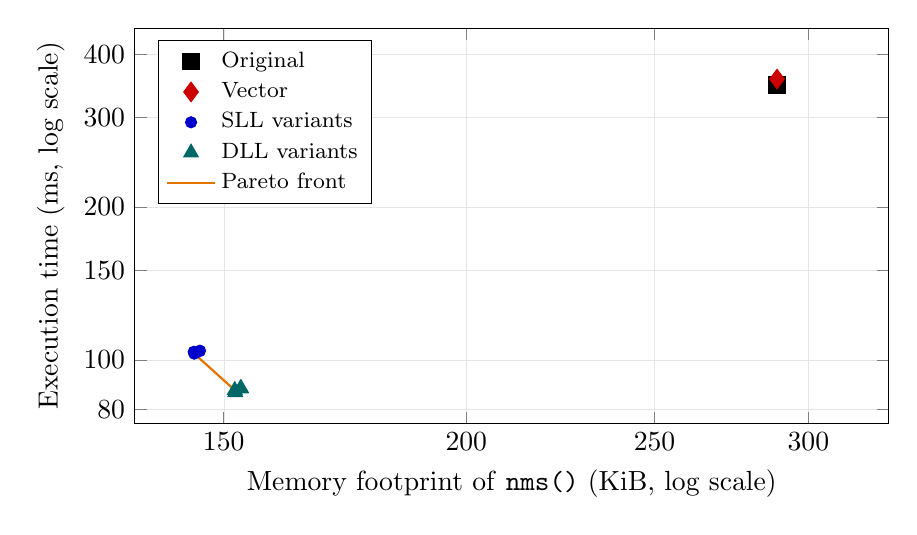
\begin{tikzpicture}
\begin{axis}[width=0.92\textwidth, height=6.6cm, xmode=log, ymode=log, log ticks with fixed point, grid=both, grid style={line width=.1pt, draw=gray!20}, legend cell align={left}, legend style={font=\footnotesize}, xlabel={Memory footprint of \texttt{nms()} (KiB, log scale)}, ylabel={Execution time (ms, log scale)}, xtick={150,200,250,300}, ytick={80,100,150,200,300,400}, xmin=135, xmax=330, ymin=75, ymax=450, legend pos=north west]
\addplot[only marks, mark=square*, mark size=3pt, color=black] coordinates {(289.00,347.539)};
\addlegendentry{Original}
\addplot[only marks, mark=diamond*, mark size=3.5pt, color=red!80!black] coordinates {(289.05,357.276)};
\addlegendentry{Vector}
\addplot[only marks, mark=*, color=blue!80!black] coordinates {(145.73,104.023) (145.83,104.266) (144.75,103.730) (144.84,102.856)};
\addlegendentry{SLL variants}
\addplot[only marks, mark=triangle*, mark size=3pt, color=teal!80!black] coordinates {(153.00,87.773) (153.09,88.000) (151.97,87.177) (152.06,86.323)};
\addlegendentry{DLL variants}
\addplot[thick, color=orange!90!black, mark=none] coordinates {(144.75,103.730) (144.84,102.856) (151.97,87.177) (152.06,86.323)};
\addlegendentry{Pareto front}
\end{axis}
\end{tikzpicture}
\caption{Όλος ο χώρος σχεδίασης (λογαριθμικοί άξονες).}
\end{subfigure}
\par\medskip
\begin{subfigure}{\textwidth}\centering
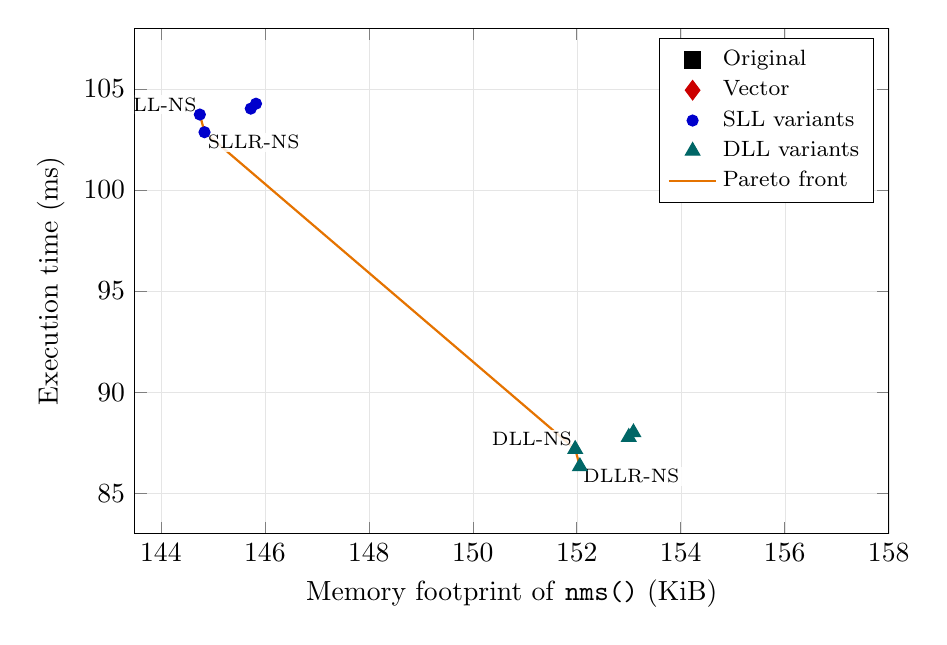
\begin{tikzpicture}
\begin{axis}[width=0.92\textwidth, height=8cm, grid=both, grid style={line width=.1pt, draw=gray!20}, legend cell align={left}, legend style={font=\footnotesize}, xlabel={Memory footprint of \texttt{nms()} (KiB)}, ylabel={Execution time (ms)}, legend pos=north east, xmin=143.5, xmax=158, ymin=83, ymax=108, legend style={at={(0.98,0.98)}, anchor=north east}]
\addplot[only marks, mark=square*, mark size=3pt, color=black] coordinates {(289.00,347.539)};
\addlegendentry{Original}
\addplot[only marks, mark=diamond*, mark size=3.5pt, color=red!80!black] coordinates {(289.05,357.276)};
\addlegendentry{Vector}
\addplot[only marks, mark=*, color=blue!80!black] coordinates {(145.73,104.023) (145.83,104.266) (144.75,103.730) (144.84,102.856)};
\addlegendentry{SLL variants}
\addplot[only marks, mark=triangle*, mark size=3pt, color=teal!80!black] coordinates {(153.00,87.773) (153.09,88.000) (151.97,87.177) (152.06,86.323)};
\addlegendentry{DLL variants}
\addplot[thick, color=orange!90!black, mark=none] coordinates {(144.75,103.730) (144.84,102.856) (151.97,87.177) (152.06,86.323)};
\addlegendentry{Pareto front}
\node[font=\scriptsize, anchor=south east, fill=white, fill opacity=0.85, text opacity=1, inner sep=1pt] at (axis cs:144.75,103.730) {SLL-NS};
\node[font=\scriptsize, anchor=north west, fill=white, fill opacity=0.85, text opacity=1, inner sep=1pt] at (axis cs:144.84,102.856) {SLLR-NS};
\node[font=\scriptsize, anchor=south east, fill=white, fill opacity=0.85, text opacity=1, inner sep=1pt] at (axis cs:151.97,87.177) {DLL-NS};
\node[font=\scriptsize, anchor=north west, fill=white, fill opacity=0.85, text opacity=1, inner sep=1pt] at (axis cs:152.06,86.323) {DLLR-NS};
\end{axis}
\end{tikzpicture}
\caption{Μεγέθυνση στην περιοχή των λιστών, με τα Pareto optimal σημεία.}
\end{subfigure}
\caption{Pareto plot του Ζητουμένου 2 (memory footprint -- χρόνος εκτέλεσης) για τις 9 δομές με glibc και την αρχική έκδοση. Η γραμμή ενώνει τις Pareto optimal λύσεις.}
\label{fig:q2}
\end{figure}

\subsubsection*{Σχολιασμός Αποτελεσμάτων Πίνακα \ref{tab:q2} και Σχήματος \ref{fig:q2}}
\begin{itemize}
    \item \textbf{Ελάχιστος χρόνος εκτέλεσης:} \en{DLLR-NS} με \en{glibc} (86.32 \en{ms}, 4.03$\times$ γρηγορότερη από την αρχική έκδοση).
    \item \textbf{Ελάχιστο \en{memory footprint}:} \en{SLL-NS} με \en{glibc} (148{,}224 \en{B}, 50\% λιγότερη μνήμη από την αρχική έκδοση).
    \item \textbf{\en{Pareto optimal} λύσεις:} \en{SLL-NS} (148{,}224 \en{B}, 103.73 \en{ms}), \en{SLLR-NS} (148{,}320 \en{B}, 102.86 \en{ms}), \en{DLL-NS} (155{,}616 \en{B}, 87.18 \en{ms}), \en{DLLR-NS} (155{,}712 \en{B}, 86.32 \en{ms}). Σε σχέση με την αρχική έκδοση, όλες οι λύσεις του \en{Pareto front} είναι ταυτόχρονα 3.3--4.0$\times$ γρηγορότερες και χρειάζονται περίπου τη μισή μνήμη.
\end{itemize}

\textbf{Γιατί ο \en{vector} είναι ο χειρότερος.} Ο \en{\texttt{ddtr::vector}} συμπεριφέρεται όπως ο \en{\texttt{std::vector}} της αρχικής έκδοσης, και τα αποτελέσματά του είναι πρακτικά ίδια (357.28 \en{ms}, 289 \en{KiB}). Κάθε \en{\texttt{erase}} μετακινεί όλα τα επόμενα στοιχεία των 152 \en{B} μια θέση πίσω ($O(k)$ ανά διαγραφή), και η \en{NMS} διαγράφει τα περισσότερα πλαίσια, οπότε ο χρόνος κυριαρχείται από αυτές τις αντιγραφές. Επιπλέον ο διπλασιασμός της χωρητικότητας αφήνει $\approx 50\%$ της μνήμης αχρησιμοποίητη.

\textbf{Γιατί οι λίστες κερδίζουν.} Η \en{\texttt{erase}} μιας λίστας απλώς αποσυνδέει έναν κόμβο ($O(1)$, χωρίς μετακίνηση δεδομένων), και η λίστα δεσμεύει ακριβώς έναν κόμβο ανά στοιχείο: 924 κόμβοι των 160 \en{B} (152 \en{B} \en{Detection} + δείκτης \en{\texttt{next}}) για την \en{SLL}, και των 168 \en{B} (+ δείκτης \en{\texttt{prev}}) για τη \en{DLL}, δηλαδή 147{,}840 και 155{,}232 \en{B} αντίστοιχα στο \en{peak}.

\textbf{Γιατί η \en{DLL} είναι γρηγορότερη από την \en{SLL}.} Η \en{\texttt{erase(it)}} χρειάζεται τον προηγούμενο κόμβο για να τον συνδέσει με τον επόμενο. Η \en{DLL} τον έχει στον δείκτη \en{\texttt{prev}}, ενώ η \en{SLL} πρέπει να τον βρει διασχίζοντας τη λίστα από την αρχή, άρα η διαγραφή της είναι $O(k)$. Η \en{DLL} πληρώνει 8 \en{B} περισσότερα ανά κόμβο ($\approx 5\%$ μνήμη) για να είναι $\approx 16\%$ γρηγορότερη. Γι' αυτό η \en{SLL} και η \en{DLL} είναι και οι δύο στο \en{Pareto front}: η μία για μνήμη, η άλλη για χρόνο.

\textbf{\en{Roving pointer} και \en{sentinel}.} Ο \en{roving pointer} κρατά τη θέση της τελευταίας πρόσβασης ώστε να επιταχύνει την πρόσβαση με δείκτη (\en{\texttt{get(n)}}). Ο βρόχος μας χρησιμοποιεί μόνο \en{iterators}, οπότε δεν ωφελείται, και οι διαφορές με/χωρίς \en{roving} είναι το πολύ $\approx 1\%$, με κόστος 96 \en{B} για τον επιπλέον δείκτη. Η αφαίρεση του κόμβου \en{sentinel} γλιτώνει έναν κενό κόμβο ανά κλάση (το \en{footprint} πέφτει κατά 1{,}008--1{,}056 \en{B}) και λίγους ελέγχους, γι' αυτό οι εκδοχές \en{no sentinel} είναι οριακά καλύτερες και στα δύο κριτήρια και καταλαμβάνουν όλο το \en{Pareto front}.

\textbf{\en{LLC misses}.} Τα \en{$\Delta$L2 refills} είναι σχεδόν ίδια για όλες τις εκδοχές ($\approx$ 185--187 χιλιάδες), αν και ο χρόνος διαφέρει κατά 4$\times$. Τα δεδομένα ενός \en{frame} (150--300 \en{KiB}) χωρούν άνετα στην \en{L2}, οπότε οι διαφορές στον χρόνο οφείλονται στον αριθμό των εντολών (μετακινήσεις στοιχείων του \en{vector}, διασχίσεις της \en{SLL}) και στην καθυστέρηση της πρόσβασης μέσω δεικτών, όχι σε \en{misses} της \en{LLC}.

% =============================================================================
\section{Ζητούμενο 3: Χρήση Διαφορετικών \en{Allocators}}
\label{sec:q3}
% =============================================================================
\subsection{Υλοποίηση}
Ο \en{allocator} είναι η δεύτερη παράμετρος κάθε δομής της \en{DDTR}: ένα \en{struct} με δύο \en{static} συναρτήσεις \en{\texttt{malloc(size)}} και \en{\texttt{free(pointer)}}, από τις οποίες η δομή παίρνει όλη τη μνήμη της (κόμβους, \en{buffers} του \en{vector}, τον προσωρινό \en{buffer} της \en{sort}). Και οι τρεις \en{allocators} μας παίρνουν μνήμη από το λειτουργικό με \en{\texttt{mmap}} σε κομμάτια του 1 \en{MiB} και επιστρέφουν διευθύνσεις ευθυγραμμισμένες στα 16 \en{B}, όπως η \en{glibc}.

\textbf{\en{Arena allocator} (\en{Listing}~\ref{lst:arena}).} Η \en{\texttt{malloc}} μετακινεί μια θέση (\en{bump pointer}) προς τα εμπρός μέσα στο τρέχον κομμάτι και, αν δεν χωράει, προχωρά στο επόμενο κομμάτι ή δεσμεύει νέο με \en{\texttt{mmap}}. Τα \en{blocks} δεν έχουν \en{header}. Η \en{\texttt{free}} δεν επιστρέφει ποτέ μεμονωμένο \en{block}: μειώνει μόνο έναν μετρητή ζωντανών \en{blocks}, και όταν μηδενιστεί η θέση επιστρέφει στην αρχή του πρώτου κομματιού. Τα κομμάτια δεν αποδεσμεύονται ποτέ, οπότε ξαναχρησιμοποιούνται στο επόμενο \en{frame}. \textbf{Διαχείριση \en{free blocks}:} δεν υπάρχει \en{free list}, η ελεύθερη μνήμη είναι ό,τι βρίσκεται μετά τη θέση, και ανακτάται μόνο όλη μαζί.

\begin{lstlisting}[caption={Arena allocator: \texttt{malloc} και \texttt{free} (\texttt{allocators/arena\_allocator.hpp}).}, label={lst:arena}]
    struct chunk {
        std::size_t size;  // of the whole chunk, this header included
        chunk* next;       // next chunk in the list
    };
    // Sizes are rounded up to 16 and the chunk header is 16 bytes, so every block that malloc
    // returns is aligned to 16 bytes, like glibc's. Blocks have no header of their own.
    static_assert(sizeof(chunk) == 16, "chunk header must be 16 bytes");

    static constexpr std::size_t MMAP_BYTES = 1 << 20;
    static inline chunk* first = nullptr;    // first chunk ever mapped
    static inline chunk* last = nullptr;     // last chunk, where new chunks are appended
    static inline chunk* current = nullptr;  // chunk the position is in
    static inline std::size_t offset = 0;    // the position, from the start of current
    static inline std::size_t live = 0;      // blocks malloc'd and not yet freed

    static void* malloc(std::size_t size) {
        std::size_t needed = (size + 15) / 16 * 16;
        if (needed == 0) needed = 16;

        // Move on to the next chunks until one has room; map a new one if none has.
        while (!current || offset + needed > current->size) {
            if (current && current->next) {
                current = current->next;
            } else {
                std::size_t bytes = (sizeof(chunk) + needed + MMAP_BYTES - 1) / MMAP_BYTES * MMAP_BYTES;
                void* memory = mmap(nullptr, bytes, PROT_READ | PROT_WRITE, MAP_PRIVATE | MAP_ANONYMOUS, -1, 0);
                if (memory == MAP_FAILED) {
                    std::fprintf(stderr, "arena: mmap of %zu bytes failed\n", bytes);
                    std::abort();
                }
#ifdef ALLOC_STATS
                mmap_bytes += bytes;
#endif
                chunk* c = (chunk*)memory;
                c->size = bytes;
                c->next = nullptr;
                if (last) last->next = c;
                else first = c;
                last = c;
                current = c;
            }
            offset = sizeof(chunk);
        }

        void* block = (char*)current + offset;
        offset += needed;
        ++live;
#ifdef ALLOC_STATS
        malloc_bytes += needed;
        if (malloc_bytes > peak_malloc_bytes) peak_malloc_bytes = malloc_bytes;
#endif
        return block;
    }

    static void free(void* pointer) {
        if (!pointer) return;
        // No single block is given back. When the last live block goes, the whole arena is
        // empty and the position goes back to the start of the first chunk.
        if (--live == 0) {
            current = first;
            offset = sizeof(chunk);
#ifdef ALLOC_STATS
            malloc_bytes = 0;
#endif
        }
    }
\end{lstlisting}

\textbf{\en{First fit}, \en{best fit} (και \en{worst fit}).} Ακολουθούν τη δομή του έτοιμου \en{worst fit}: κάθε \en{block} έχει \en{header} 16 \en{B} (\en{\texttt{size}} και \en{\texttt{next}}), ώστε η \en{\texttt{free}} να βρίσκει το μέγεθος από τον δείκτη (\en{\texttt{(header*)pointer - 1}}). \textbf{Διαχείριση \en{free blocks}:} τα ελεύθερα \en{blocks} βρίσκονται σε μια απλά συνδεδεμένη \en{free list} ταξινομημένη κατά διεύθυνση, τα δεσμευμένα δεν ανήκουν σε καμία λίστα. Η \en{\texttt{free}} (συνάρτηση \en{\texttt{insert}}) βάζει το \en{block} στη σωστή θέση της λίστας και το συγχωνεύει (\en{coalescing}) με τα γειτονικά ελεύθερα \en{blocks}, ώστε να μη δημιουργείται εξωτερικός κατακερματισμός από γειτονικά μικρά κομμάτια. Οι τρεις διαφέρουν μόνο στο ποιο ελεύθερο \en{block} επιλέγει η \en{\texttt{malloc}}:
\begin{itemize}
    \item \en{\textbf{first fit}}: το πρώτο (κατά διεύθυνση) αρκετά μεγάλο \en{block};
    \item \en{\textbf{best fit}}: το μικρότερο αρκετά μεγάλο \en{block} (σταματά νωρίτερα αν βρει ακριβές ταίριασμα);
    \item \en{\textbf{worst fit}}: το μεγαλύτερο \en{block}.
\end{itemize}
Το νέο \en{block} κόβεται από το τέλος του ελεύθερου \en{block}, ώστε αυτό να κρατά τη θέση του στη λίστα. Αν το υπόλοιπο θα ήταν μικρότερο από 32 \en{B} (\en{header} + 16 \en{B}), δίνεται όλο το \en{block} και αφαιρείται από τη λίστα. Αν κανένα \en{block} δεν χωρά, δεσμεύεται νέο κομμάτι με \en{\texttt{mmap}} και εισάγεται στη λίστα.

\begin{lstlisting}[caption={First fit allocator: \texttt{malloc}, \texttt{free} και \texttt{insert} με coalescing (\texttt{allocators/first\_fit\_allocator.hpp}).}, label={lst:firstfit}]
struct first_fit {
    // In front of every block, as in worst_fit. 16 bytes, and all sizes are multiples of 16,
    // so the memory that malloc returns is aligned to 16 bytes.
    struct header {
        std::size_t size;  // of the whole block, header included
        header* next;      // next free block (only while this block is free)
    };

    static constexpr std::size_t MMAP_BYTES = 1 << 20;
    // A free block smaller than this is not worth keeping: header + 16 bytes of data.
    static constexpr std::size_t MIN_BLOCK = sizeof(header) + 16;
    // Free blocks, sorted by address. Allocated blocks are in no list.
    static inline header* free_list = nullptr;

    static void* malloc(std::size_t size) {
        std::size_t needed = (sizeof(header) + size + 15) / 16 * 16;

        // The first free block in address order that is big enough.
        header* before = nullptr;
        header* found = free_list;
        while (found && found->size < needed) {
            before = found;
            found = found->next;
        }

        if (!found) {
            std::size_t bytes = (needed + MMAP_BYTES - 1) / MMAP_BYTES * MMAP_BYTES;
            void* memory = mmap(nullptr, bytes, PROT_READ | PROT_WRITE, MAP_PRIVATE | MAP_ANONYMOUS, -1, 0);
            if (memory == MAP_FAILED) {
                std::fprintf(stderr, "first_fit: mmap of %zu bytes failed\n", bytes);
                std::abort();
            }
#ifdef ALLOC_STATS
            mmap_bytes += bytes;
#endif
            header* fresh = (header*)memory;
            fresh->size = bytes;
            insert(fresh);  // may merge it with the free block at the end of the last piece
            before = nullptr;
            found = free_list;
            while (found && found->size < needed) {
                before = found;
                found = found->next;
            }
        }

        header* block;
        if (found->size - needed >= MIN_BLOCK) {
            // Cut the new block from the end, so the free block keeps its place in the list.
            found->size -= needed;
            block = (header*)((char*)found + found->size);
            block->size = needed;
        } else {
            // What would be left is too small to be a block: hand out the whole block.
            if (before) before->next = found->next;
            else free_list = found->next;
            block = found;
        }
#ifdef ALLOC_STATS
        malloc_bytes += block->size;
        if (malloc_bytes > peak_malloc_bytes) peak_malloc_bytes = malloc_bytes;
#endif
        return block + 1;
    }

    static void free(void* pointer) {
        if (!pointer) return;
        header* block = (header*)pointer - 1;  // one header (16 bytes) back
#ifdef ALLOC_STATS
        malloc_bytes -= block->size;
#endif
        insert(block);
    }

    // Puts a block in the free list, in address order, and merges it with the free blocks
    // right before and after it.
    static void insert(header* block) {
        header* before = nullptr;
        header* after = free_list;
        while (after && after < block) {
            before = after;
            after = after->next;
        }
        block->next = after;
        if (before) before->next = block;
        else free_list = block;

        if (after && (char*)block + block->size == (char*)after) {
            block->size += after->size;
            block->next = after->next;
        }
        if (before && (char*)before + before->size == (char*)block) {
            before->size += block->size;
            before->next = block->next;
        }
    }
\end{lstlisting}

\begin{lstlisting}[caption={Best fit allocator: η αναζήτηση του μικρότερου block που χωρά (\texttt{allocators/best\_fit\_allocator.hpp}), η \texttt{malloc} και η \texttt{free} είναι ίδιες με του first fit.}, label={lst:bestfit}]

    // The smallest free block of at least `needed` bytes, and the block before it in the list
    // (nullptr if it is the first). Stops early on an exact fit.
    static header* find(std::size_t needed, header*& best_before) {
        header* best = nullptr;
        best_before = nullptr;
        header* before = nullptr;
        for (header* b = free_list; b; before = b, b = b->next) {
            if (b->size >= needed && (!best || b->size < best->size)) {
                best = b;
                best_before = before;
                if (b->size == needed) break;
            }
        }
        return best;
    }
\end{lstlisting}

\textbf{Μετρητές \en{\texttt{ALLOC\_STATS}}.} Μέσα σε \en{\texttt{\#ifdef ALLOC\_STATS}} κάθε \en{allocator} μετρά τα \en{bytes} που πήρε από την \en{\texttt{mmap}} (\en{\texttt{mmap\_bytes}}) και τα \en{bytes} των \en{blocks} που είναι δεσμευμένα (με το \en{header} τους), κρατώντας τη μέγιστη τιμή (\en{\texttt{malloc\_bytes}}). Για τον \en{arena} μετρά τα \en{bytes} που χρησιμοποιήθηκαν από την τελευταία επιστροφή της θέσης στην αρχή. Οι μετρήσεις χρόνου έγιναν με εκτελέσιμα χωρίς το \en{flag}, ώστε οι μετρητές να μην επηρεάζουν τον χρόνο.

\textbf{Έλεγχοι.} Εκτός από το \en{\texttt{-DVALIDATE}} για όλους τους συνδυασμούς, κάθε \en{allocator} πέρασε ένα \en{stress test} με 600{,}000 τυχαίες \en{\texttt{malloc}}/\en{\texttt{free}} μεγεθών 0--20{,}000 \en{B}, στο οποίο κάθε \en{block} γεμίζει με το δικό του μοτίβο και ελέγχεται πριν αποδεσμευτεί (εντοπίζει επικαλυπτόμενα \en{blocks} ή κατεστραμμένη \en{free list}).

\subsection{Αποτελέσματα}
\begin{table}[H]
\centering
\caption{Mean execution time (ms, 3 executions $\times$ 20 runs) for every DDT and allocator on the AUP-ZU3. The glibc column is Table~\ref{tab:q2}. Bold: the fastest allocator of each DDT.}
\label{tab:q3_time}
\begin{tabular}{@{}lrrrrr@{}}
\toprule
DDT & glibc & arena & first fit & best fit & worst fit \\
\midrule
Vector & 357.28 & 352.30 & 351.79 & \textbf{351.28} & 352.25 \\
SLL & 104.02 & \textbf{72.71} & 82.76 & 83.31 & 85.33 \\
DLL & 87.77 & \textbf{55.59} & 63.74 & 64.34 & 65.85 \\
SLLR & 104.27 & \textbf{72.79} & 83.03 & 83.57 & 85.57 \\
DLLR & 88.00 & \textbf{55.74} & 63.84 & 64.43 & 65.94 \\
SLL-NS & 103.73 & \textbf{71.55} & 81.67 & 82.21 & 81.84 \\
DLL-NS & 87.18 & \textbf{54.87} & 62.34 & 62.77 & 62.10 \\
SLLR-NS & 102.86 & \textbf{71.44} & 82.16 & 82.55 & 82.20 \\
DLLR-NS & 86.32 & \textbf{55.02} & 62.54 & 63.04 & 62.32 \\
\bottomrule
\end{tabular}
\end{table}

\begin{table}[H]
\centering
\caption{Memory footprint (bytes) of \texttt{nms()}. glibc: Massif; own allocators: peak \texttt{malloc\_bytes} of \texttt{-DALLOC\_STATS} (blocks with their headers). First, best and worst fit gave identical values. \texttt{mmap\_bytes} was 1{,}048{,}576 B (1 MiB) for every combination.}
\label{tab:q3_mem}
\begin{tabular}{@{}lrrr@{}}
\toprule
DDT & glibc (Massif) & arena & first / best / worst fit \\
\midrule
Vector & 295{,}992 & 505{,}632 & 295{,}616 \\
SLL & 149{,}232 & 149{,}760 & 163{,}680 \\
DLL & 156{,}672 & 164{,}736 & 178{,}560 \\
SLLR & 149{,}328 & 149{,}760 & 163{,}680 \\
DLLR & 156{,}768 & 164{,}736 & 178{,}560 \\
SLL-NS & 148{,}224 & 147{,}840 & 162{,}624 \\
DLL-NS & 155{,}616 & 162{,}624 & 177{,}408 \\
SLLR-NS & 148{,}320 & 147{,}840 & 162{,}624 \\
DLLR-NS & 155{,}712 & 162{,}624 & 177{,}408 \\
\bottomrule
\end{tabular}
\end{table}

\begin{table}[H]
\centering
\caption{$\Delta$L2 refills (\texttt{l2d\_cache\_refill}, runs=1 $-$ runs=0, mean of 20 perf runs) for every DDT and allocator.}
\label{tab:q3_l2}
\begin{tabular}{@{}lrrrrr@{}}
\toprule
DDT & glibc & arena & first fit & best fit & worst fit \\
\midrule
Vector & 187{,}208 & 206{,}553 & 192{,}394 & 187{,}779 & 191{,}306 \\
SLL & 185{,}572 & 186{,}268 & 186{,}873 & 186{,}368 & 185{,}573 \\
DLL & 184{,}951 & 184{,}693 & 187{,}236 & 186{,}880 & 185{,}752 \\
SLLR & 185{,}909 & 185{,}408 & 186{,}021 & 185{,}824 & 185{,}452 \\
DLLR & 186{,}440 & 185{,}462 & 185{,}461 & 186{,}438 & 186{,}143 \\
SLL-NS & 185{,}120 & 184{,}829 & 185{,}787 & 184{,}757 & 186{,}585 \\
DLL-NS & 185{,}561 & 185{,}676 & 184{,}317 & 184{,}717 & 186{,}089 \\
SLLR-NS & 185{,}542 & 184{,}807 & 185{,}985 & 185{,}226 & 184{,}606 \\
DLLR-NS & 185{,}779 & 186{,}166 & 186{,}007 & 186{,}021 & 186{,}053 \\
\bottomrule
\end{tabular}
\end{table}

\begin{figure}[H]
\centering
\begin{subfigure}{\textwidth}\centering
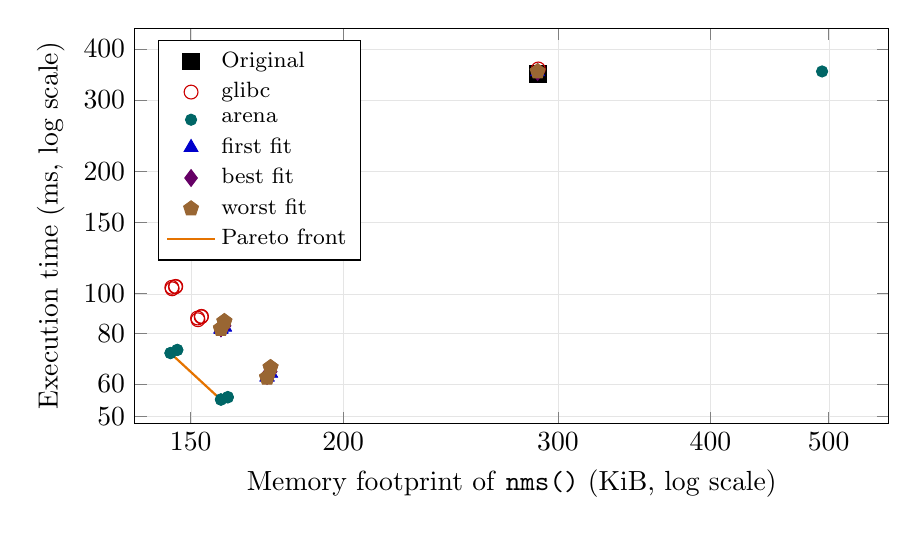
\begin{tikzpicture}
\begin{axis}[width=0.92\textwidth, height=6.6cm, xmode=log, ymode=log, log ticks with fixed point, grid=both, grid style={line width=.1pt, draw=gray!20}, legend cell align={left}, legend style={font=\footnotesize}, xlabel={Memory footprint of \texttt{nms()} (KiB, log scale)}, ylabel={Execution time (ms, log scale)}, xtick={150,200,300,400,500}, ytick={50,60,80,100,150,200,300,400}, xmin=135, xmax=560, ymin=48, ymax=450, legend pos=north west]
\addplot[only marks, mark=square*, mark size=3pt, color=black] coordinates {(289.00,347.539)};
\addlegendentry{Original}
\addplot[only marks, mark=o, mark size=2.5pt, color=red!80!black] coordinates {(289.05,357.276) (145.73,104.023) (153.00,87.773) (145.83,104.266) (153.09,88.000) (144.75,103.730) (151.97,87.177) (144.84,102.856) (152.06,86.323)};
\addlegendentry{glibc}
\addplot[only marks, mark=*, color=teal!80!black] coordinates {(493.78,352.303) (146.25,72.708) (160.88,55.587) (146.25,72.791) (160.88,55.744) (144.38,71.554) (158.81,54.865) (144.38,71.436) (158.81,55.018)};
\addlegendentry{arena}
\addplot[only marks, mark=triangle*, mark size=2.8pt, color=blue!80!black] coordinates {(288.69,351.790) (159.84,82.756) (174.38,63.737) (159.84,83.032) (174.38,63.842) (158.81,81.666) (173.25,62.340) (158.81,82.160) (173.25,62.541)};
\addlegendentry{first fit}
\addplot[only marks, mark=diamond*, mark size=3pt, color=violet!80!black] coordinates {(288.69,351.280) (159.84,83.312) (174.38,64.339) (159.84,83.569) (174.38,64.427) (158.81,82.209) (173.25,62.768) (158.81,82.546) (173.25,63.037)};
\addlegendentry{best fit}
\addplot[only marks, mark=pentagon*, mark size=2.8pt, color=brown!80!black] coordinates {(288.69,352.251) (159.84,85.334) (174.38,65.849) (159.84,85.572) (174.38,65.935) (158.81,81.843) (173.25,62.102) (158.81,82.198) (173.25,62.321)};
\addlegendentry{worst fit}
\addplot[thick, color=orange!90!black, mark=none] coordinates {(144.38,71.436) (158.81,54.865)};
\addlegendentry{Pareto front}
\end{axis}
\end{tikzpicture}
\caption{Όλος ο χώρος σχεδίασης (λογαριθμικοί άξονες).}
\end{subfigure}
\par\medskip
\begin{subfigure}{\textwidth}\centering
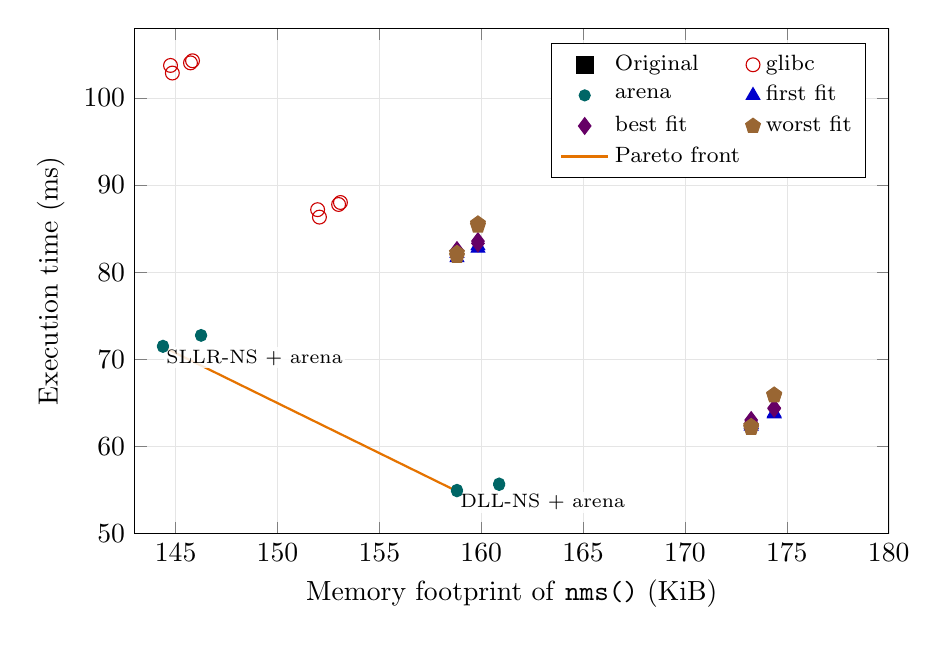
\begin{tikzpicture}
\begin{axis}[width=0.92\textwidth, height=8cm, grid=both, grid style={line width=.1pt, draw=gray!20}, legend cell align={left}, legend style={font=\footnotesize}, xlabel={Memory footprint of \texttt{nms()} (KiB)}, ylabel={Execution time (ms)}, legend pos=north east, xmin=143, xmax=180, ymin=50, ymax=108, legend columns=2]
\addplot[only marks, mark=square*, mark size=3pt, color=black] coordinates {(289.00,347.539)};
\addlegendentry{Original}
\addplot[only marks, mark=o, mark size=2.5pt, color=red!80!black] coordinates {(289.05,357.276) (145.73,104.023) (153.00,87.773) (145.83,104.266) (153.09,88.000) (144.75,103.730) (151.97,87.177) (144.84,102.856) (152.06,86.323)};
\addlegendentry{glibc}
\addplot[only marks, mark=*, color=teal!80!black] coordinates {(493.78,352.303) (146.25,72.708) (160.88,55.587) (146.25,72.791) (160.88,55.744) (144.38,71.554) (158.81,54.865) (144.38,71.436) (158.81,55.018)};
\addlegendentry{arena}
\addplot[only marks, mark=triangle*, mark size=2.8pt, color=blue!80!black] coordinates {(288.69,351.790) (159.84,82.756) (174.38,63.737) (159.84,83.032) (174.38,63.842) (158.81,81.666) (173.25,62.340) (158.81,82.160) (173.25,62.541)};
\addlegendentry{first fit}
\addplot[only marks, mark=diamond*, mark size=3pt, color=violet!80!black] coordinates {(288.69,351.280) (159.84,83.312) (174.38,64.339) (159.84,83.569) (174.38,64.427) (158.81,82.209) (173.25,62.768) (158.81,82.546) (173.25,63.037)};
\addlegendentry{best fit}
\addplot[only marks, mark=pentagon*, mark size=2.8pt, color=brown!80!black] coordinates {(288.69,352.251) (159.84,85.334) (174.38,65.849) (159.84,85.572) (174.38,65.935) (158.81,81.843) (173.25,62.102) (158.81,82.198) (173.25,62.321)};
\addlegendentry{worst fit}
\addplot[thick, color=orange!90!black, mark=none] coordinates {(144.38,71.436) (158.81,54.865)};
\addlegendentry{Pareto front}
\node[font=\scriptsize, anchor=north west, fill=white, fill opacity=0.85, text opacity=1, inner sep=1pt] at (axis cs:144.38,71.436) {SLLR-NS + arena};
\node[font=\scriptsize, anchor=north west, fill=white, fill opacity=0.85, text opacity=1, inner sep=1pt] at (axis cs:158.81,54.865) {DLL-NS + arena};
\end{axis}
\end{tikzpicture}
\caption{Μεγέθυνση στην περιοχή των λιστών, με τα Pareto optimal σημεία.}
\end{subfigure}
\caption{Pareto plot του Ζητουμένου 3 για όλους τους συνδυασμούς δομής -- allocator, μαζί με τις υλοποιήσεις glibc και την αρχική έκδοση. Η γραμμή ενώνει τις Pareto optimal λύσεις.}
\label{fig:q3}
\end{figure}

\subsubsection*{Σχολιασμός Αποτελεσμάτων Ζητουμένου 3}
\begin{itemize}
    \item \textbf{\en{Pareto optimal} λύσεις:} \en{SLLR-NS} με \en{arena} (147{,}840 \en{B}, 71.44 \en{ms}), \en{DLL-NS} με \en{arena} (162{,}624 \en{B}, 54.87 \en{ms}). Και οι δύο χρησιμοποιούν τον \en{arena allocator}.
    \item \textbf{Σε σχέση με την αρχική υλοποίηση:} η ταχύτερη λύση είναι 6.3$\times$ γρηγορότερη από την αρχική έκδοση με το 55\% της μνήμης, και 36\% γρηγορότερη από την καλύτερη λύση του Ζητουμένου 2 με \en{glibc}.
\end{itemize}

\textbf{\en{Arena}: ο ταχύτερος.} Για όλες τις λίστες ο \en{arena} είναι ο ταχύτερος \en{allocator}, 30--37\% γρηγορότερος από τη \en{glibc}. Η \en{\texttt{malloc}} του είναι μια πρόσθεση και ένας έλεγχος, και η \en{\texttt{free}} μια μείωση μετρητή, χωρίς αναζήτηση και χωρίς \en{headers}. Επιπλέον οι κόμβοι δεσμεύονται συνεχόμενα στη σειρά που προστίθενται στη λίστα, οπότε η διάσχιση της λίστας γίνεται σχεδόν σειριακά στη μνήμη (καλή χωρική τοπικότητα). Η \en{NMS} ταιριάζει ιδανικά σε \en{arena}: όλη η μνήμη ενός \en{frame} ελευθερώνεται μαζί στο τέλος της \en{\texttt{nms()}}, οπότε η θέση επιστρέφει στην αρχή σε κάθε \en{frame}. Οι λίστες με \en{arena} έχουν και το μικρότερο \en{footprint}, αφού δεν υπάρχει \en{header} 16 \en{B} ανά κόμβο.

\textbf{Το μειονέκτημα του \en{arena}: ο \en{vector}.} Ο \en{arena} δεν ξαναχρησιμοποιεί μεμονωμένα \en{blocks}. Όταν ο \en{vector} μεγαλώνει, ο παλιός \en{buffer} του ελευθερώνεται αλλά η μνήμη του δεν επιστρέφει μέχρι το τέλος του \en{frame}, οπότε στο \en{peak} συνυπάρχουν οι διαδοχικοί \en{buffers} ($1 + \tfrac12 + \tfrac14 + \dots$ της τελικής χωρητικότητας): 505{,}632 \en{B} αντί για 295{,}616 \en{B} (1.7$\times$). Αυτό φαίνεται και στα \en{$\Delta$L2 refills}, που είναι τα μεγαλύτερα όλου του πίνακα (206{,}553), γιατί κάθε νέος \en{buffer} πιάνει μνήμη που δεν έχει αγγιχτεί πρόσφατα.

\textbf{\en{First}, \en{best} και \en{worst fit}.} Δίνουν \textbf{ακριβώς το ίδιο} \en{footprint}, γιατί όλα τα \en{blocks} μιας δομής έχουν το ίδιο μέγεθος (ένας κόμβος), οπότε όποιο ελεύθερο \en{block} κι αν επιλεγεί, το αποτέλεσμα στη μνήμη είναι ίδιο, οι πολιτικές διαφέρουν μόνο στον χρόνο αναζήτησης. Στις λίστες με \en{sentinel} η σειρά είναι η αναμενόμενη: ο \en{first fit} σταματά στο πρώτο ταίριασμα και είναι ο ταχύτερος, ο \en{best fit} ελέγχει περισσότερα \en{blocks}, και ο \en{worst fit}, που διασχίζει πάντα όλη την \en{free list}, είναι ο πιο αργός. Στις εκδοχές \en{no sentinel} οι τρεις απέχουν λιγότερο από 1\%, γιατί η \en{free list} είναι πολύ μικρή και η αναζήτηση δεν κοστίζει σχεδόν τίποτα. Και οι τρεις είναι όμως γρηγορότεροι από τη \en{glibc} (π.χ. \en{DLL}: 63.7 έναντι 87.8 \en{ms}): είναι απλούστεροι (χωρίς \en{thread safety}, χωρίς \en{bins}), και επειδή όλοι οι κόμβοι ενός \en{frame} ελευθερώνονται και συγχωνεύονται ξανά, η \en{free list} μένει πολύ μικρή και η αναζήτηση φθηνή.

\textbf{Μετρητές \en{\texttt{ALLOC\_STATS}}: τι παρατηρούμε.} Το \en{\texttt{mmap\_bytes}} είναι 1 \en{MiB} σε όλους τους συνδυασμούς: το πιο φορτωμένο \en{frame} χωρά σε ένα κομμάτι, ενώ η πραγματική ανάγκη είναι 145--494 \en{KiB}. Άρα από τη σκοπιά του λειτουργικού το \en{footprint} καθορίζεται από το μέγεθος του κομματιού (\en{\texttt{MMAP\_BYTES}}) και όχι από τη δομή, με μικρότερα κομμάτια θα ήταν πιο κοντά στο \en{\texttt{malloc\_bytes}}, με κόστος περισσότερες κλήσεις \en{\texttt{mmap}}. Το \en{Massif} δεν βλέπει καθόλου αυτή τη μνήμη, γι' αυτό χρειάζονται οι μετρητές μέσα στον \en{allocator}. Σημειώνουμε ότι τα νούμερα \en{glibc} (\en{Massif}) δεν περιλαμβάνουν το \en{header} της \en{\texttt{malloc}} ($\approx$ 8--16 \en{B} ανά \en{block}, που το \en{Massif} δίνει χωριστά ως \en{extra heap}: 7.5 \en{KB} για την \en{SLL}, 15 \en{KB} για τη \en{DLL}), ενώ οι δικοί μας μετρητές το περιλαμβάνουν, με αυτό υπόψη η διαφορά της \en{glibc} από τους \en{first/best/worst fit} πέφτει σε λίγα τοις εκατό.

\textbf{\en{LLC misses}.} Όπως και στο Ζητούμενο 2, τα \en{$\Delta$L2 refills} είναι σχεδόν σταθερά ($\approx$ 184--187 χιλιάδες) για όλους τους συνδυασμούς εκτός από τον \en{vector} με \en{arena} και \en{first/worst fit} (191--207 χιλιάδες), οπότε η επιλογή \en{allocator} επηρεάζει τον χρόνο κυρίως μέσω του κόστους των \en{\texttt{malloc}/\texttt{free}} και της τοπικότητας στην \en{L1}, όχι μέσω της \en{LLC}.

\textbf{Ποιον \en{allocator} θα προτιμούσαμε.} Τον \textbf{\en{arena}}, σε συνδυασμό με λίστα: είναι ο ταχύτερος και, για τις λίστες, ο πιο οικονομικός σε μνήμη, και ταιριάζει στη ζωή των δεδομένων της \en{NMS}, που ζουν μόνο μέσα σε μία κλήση της \en{\texttt{nms()}}. Θα τον αποφεύγαμε μόνο με τον \en{vector} ή σε εφαρμογές όπου η μνήμη δεν ελευθερώνεται ποτέ ολόκληρη. Από τους \en{allocators} με \en{free list}, ο \en{first fit} είναι η καλύτερη επιλογή εδώ, αφού με \en{blocks} ίδιου μεγέθους οι πιο ακριβές αναζητήσεις του \en{best/worst fit} δεν κερδίζουν τίποτα σε μνήμη.

% =============================================================================
\section{Ζητούμενο 4: Χρήση \en{Flag} αντί για \en{Erase}}
% =============================================================================
\subsection{Υλοποίηση}
Η νέα εκδοχή (\en{Listing}~\ref{lst:q4}) γράφτηκε μετά το \en{\texttt{dets.sort()}} μέσα σε \en{\texttt{\#ifdef NMS\_FLAG}}, ενώ ο βρόχος του Ζητουμένου 2 έμεινε στο \en{\texttt{\#else}}. Δηλώσαμε \en{\texttt{using Flags = ddtr::vector<unsigned char, sel\_alloc\_dets>;}}, ώστε και η μνήμη των \en{flags} να περνά από τον ίδιο \en{allocator}. Το \en{vector} έχει ένα \en{byte} ανά πλαίσιο (1 = απορρίφθηκε) και δεσμεύεται με \en{\texttt{reserve}} στο ακριβές μέγεθος, ώστε να μη μεγαλώνει. Τα πλαίσια δεν αφαιρούνται ποτέ από τη δομή: ο εξωτερικός βρόχος παραλείπει όσα έχουν \en{flag}, και ο εσωτερικός σημαδεύει όσα επικαλύπτονται. Οι δείκτες \en{\texttt{i}}, \en{\texttt{j}} των \en{flags} προχωρούν μαζί με τους \en{iterators}, οπότε δεν γίνεται πρόσβαση με δείκτη στη λίστα. Η ορθότητα ελέγχθηκε με \en{\texttt{-DNMS\_FLAG -DVALIDATE}} για όλους τους 45 συνδυασμούς.

\begin{lstlisting}[caption={Η εκδοχή με flags (Ζητούμενο 4) στην \texttt{nms()}.}, label={lst:q4}]
// Q4: one flag per box (1 = rejected), through the same allocator as Dets.
using Flags = ddtr::vector<unsigned char, sel_alloc_dets>;

// ... inside nms(), for every class, after dets.sort():
#ifdef NMS_FLAG
    // Q4: the rejected boxes are not erased, only flagged; dets never changes.
    // removed[i] belongs to the i-th box in sorted order, so i and j count along with the
    // iterators.
    const std::size_t count = dets.size();
    Flags removed;
    removed.reserve(count);
    removed.resize(count, 0);
    std::size_t i = 0;
    for (auto it_m = dets.begin(); it_m != dets.end(); ++it_m, ++i) {
      if (removed[i]) continue;
      auto& item = *it_m;
      res.push_back(item);
      auto it_n = it_m;
      ++it_n;
      for (std::size_t j = i + 1; it_n != dets.end(); ++it_n, ++j)
        if (!removed[j] && iou(item.bbox, it_n->bbox) > nms_thresh)
          removed[j] = 1;
    }
#else
    // ... the erase loop of Q2 ...
#endif
\end{lstlisting}

\subsection{Αποτελέσματα}
\begin{table}[H]
\centering
\caption{\texttt{-DNMS\_FLAG}: mean execution time (ms, 3 executions $\times$ 20 runs) for every DDT and allocator. In parentheses: change with respect to the erase version of Table~\ref{tab:q3_time}. Bold: the fastest allocator of each DDT.}
\label{tab:q4_time}
\begin{tabular}{@{}lccccc@{}}
\toprule
DDT & glibc & arena & first fit & best fit & worst fit \\
\midrule
Vector & 89.02 \scriptsize(-75\%) & 83.02 \scriptsize(-76\%) & 82.78 \scriptsize(-76\%) & \textbf{82.51} \scriptsize(-77\%) & 83.26 \scriptsize(-76\%) \\
SLL & 89.27 \scriptsize(-14\%) & \textbf{60.57} \scriptsize(-17\%) & 69.91 \scriptsize(-16\%) & 70.55 \scriptsize(-15\%) & 72.37 \scriptsize(-15\%) \\
DLL & 95.00 \scriptsize(+8\%) & \textbf{63.82} \scriptsize(+15\%) & 71.65 \scriptsize(+12\%) & 72.60 \scriptsize(+13\%) & 74.11 \scriptsize(+13\%) \\
SLLR & 88.75 \scriptsize(-15\%) & \textbf{60.54} \scriptsize(-17\%) & 69.93 \scriptsize(-16\%) & 70.55 \scriptsize(-16\%) & 72.55 \scriptsize(-15\%) \\
DLLR & 94.27 \scriptsize(+7\%) & \textbf{63.93} \scriptsize(+15\%) & 71.68 \scriptsize(+12\%) & 72.35 \scriptsize(+12\%) & 74.18 \scriptsize(+13\%) \\
SLL-NS & 87.31 \scriptsize(-16\%) & \textbf{59.17} \scriptsize(-17\%) & 68.35 \scriptsize(-16\%) & 68.79 \scriptsize(-16\%) & 68.46 \scriptsize(-16\%) \\
DLL-NS & 92.88 \scriptsize(+7\%) & \textbf{62.42} \scriptsize(+14\%) & 69.82 \scriptsize(+12\%) & 70.23 \scriptsize(+12\%) & 69.54 \scriptsize(+12\%) \\
SLLR-NS & 88.42 \scriptsize(-14\%) & \textbf{58.95} \scriptsize(-17\%) & 68.54 \scriptsize(-17\%) & 68.90 \scriptsize(-17\%) & 68.53 \scriptsize(-17\%) \\
DLLR-NS & 94.07 \scriptsize(+9\%) & \textbf{62.28} \scriptsize(+13\%) & 69.94 \scriptsize(+12\%) & 70.38 \scriptsize(+12\%) & 69.75 \scriptsize(+12\%) \\
\bottomrule
\end{tabular}
\end{table}

\begin{table}[H]
\centering
\caption{\texttt{-DNMS\_FLAG}: memory footprint (bytes) of \texttt{nms()} (glibc: Massif; own allocators: peak \texttt{malloc\_bytes}; first, best and worst fit identical) and $\Delta$L2 refills (range over the 5 allocators).}
\label{tab:q4_mem}
\begin{tabular}{@{}lrrrr@{}}
\toprule
DDT & glibc (Massif) & arena & first / best / worst fit & $\Delta$L2 refills (min--max) \\
\midrule
Vector & 295{,}992 & 506{,}496 & 295{,}616 & 186{,}476--193{,}023 \\
SLL & 149{,}875 & 150{,}736 & 164{,}352 & 184{,}632--186{,}380 \\
DLL & 157{,}315 & 165{,}712 & 179{,}232 & 184{,}027--186{,}673 \\
SLLR & 149{,}971 & 150{,}736 & 164{,}352 & 183{,}970--186{,}623 \\
DLLR & 157{,}411 & 165{,}712 & 179{,}232 & 185{,}208--186{,}645 \\
SLL-NS & 148{,}867 & 148{,}816 & 163{,}296 & 183{,}623--186{,}395 \\
DLL-NS & 156{,}259 & 163{,}600 & 178{,}080 & 184{,}633--186{,}633 \\
SLLR-NS & 148{,}963 & 148{,}816 & 163{,}296 & 185{,}073--188{,}008 \\
DLLR-NS & 156{,}355 & 163{,}600 & 178{,}080 & 184{,}821--186{,}251 \\
\bottomrule
\end{tabular}
\end{table}

\begin{table}[H]
\centering
\caption{\texttt{-DNMS\_FLAG -DALLOC\_STATS}: fragmentation of the own allocators. \texttt{mmap\_bytes} = 1{,}048{,}576 B in every case. Use = \texttt{malloc\_bytes} / \texttt{mmap\_bytes}; header overhead = share of \texttt{malloc\_bytes} that is block headers and rounding (internal fragmentation), relative to arena, which has no headers (not meaningful for Vector, where arena keeps the old buffers).}
\label{tab:q4_frag}
\begin{tabular}{@{}lrrrr@{}}
\toprule
DDT & arena: use of mmap & fit: use of mmap & fit: header overhead & unused mmap (fit) \\
\midrule
Vector & 48.3\% & 28.2\% & -- & 71.8\% \\
SLL & 14.4\% & 15.7\% & 8.3\% & 84.3\% \\
DLL & 15.8\% & 17.1\% & 7.5\% & 82.9\% \\
SLLR & 14.4\% & 15.7\% & 8.3\% & 84.3\% \\
DLLR & 15.8\% & 17.1\% & 7.5\% & 82.9\% \\
SLL-NS & 14.2\% & 15.6\% & 8.9\% & 84.4\% \\
DLL-NS & 15.6\% & 17.0\% & 8.1\% & 83.0\% \\
SLLR-NS & 14.2\% & 15.6\% & 8.9\% & 84.4\% \\
DLLR-NS & 15.6\% & 17.0\% & 8.1\% & 83.0\% \\
\bottomrule
\end{tabular}
\end{table}

\begin{figure}[H]
\centering
\begin{subfigure}{\textwidth}\centering
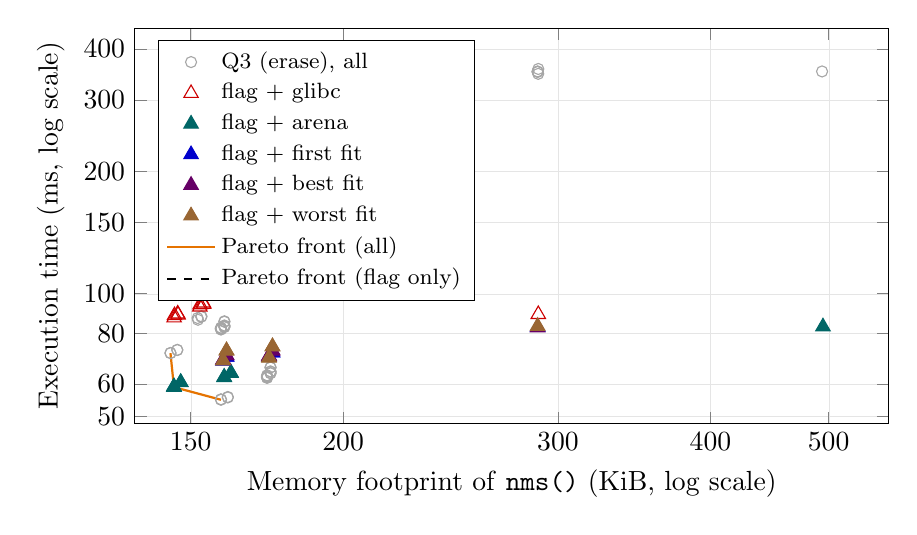
\begin{tikzpicture}
\begin{axis}[width=0.92\textwidth, height=6.6cm, xmode=log, ymode=log, log ticks with fixed point, grid=both, grid style={line width=.1pt, draw=gray!20}, legend cell align={left}, legend style={font=\footnotesize}, xlabel={Memory footprint of \texttt{nms()} (KiB, log scale)}, ylabel={Execution time (ms, log scale)}, xtick={150,200,300,400,500}, ytick={50,60,80,100,150,200,300,400}, xmin=135, xmax=560, ymin=48, ymax=450, legend pos=north west]
\addplot[only marks, mark=o, mark size=2pt, color=gray!70] coordinates {(289.00,347.539) (289.05,357.276) (145.73,104.023) (153.00,87.773) (145.83,104.266) (153.09,88.000) (144.75,103.730) (151.97,87.177) (144.84,102.856) (152.06,86.323) (493.78,352.303) (288.69,351.790) (288.69,351.280) (288.69,352.251) (146.25,72.708) (159.84,82.756) (159.84,83.312) (159.84,85.334) (160.88,55.587) (174.38,63.737) (174.38,64.339) (174.38,65.849) (146.25,72.791) (159.84,83.032) (159.84,83.569) (159.84,85.572) (160.88,55.744) (174.38,63.842) (174.38,64.427) (174.38,65.935) (144.38,71.554) (158.81,81.666) (158.81,82.209) (158.81,81.843) (158.81,54.865) (173.25,62.340) (173.25,62.768) (173.25,62.102) (144.38,71.436) (158.81,82.160) (158.81,82.546) (158.81,82.198) (158.81,55.018) (173.25,62.541) (173.25,63.037) (173.25,62.321)};
\addlegendentry{Q3 (erase), all}
\addplot[only marks, mark=triangle, mark size=3pt, color=red!80!black] coordinates {(289.05,89.016) (146.36,89.268) (153.63,95.000) (146.46,88.751) (153.72,94.268) (145.38,87.310) (152.60,92.880) (145.47,88.421) (152.69,94.067)};
\addlegendentry{flag + glibc}
\addplot[only marks, mark=triangle*, mark size=3pt, color=teal!80!black] coordinates {(494.62,83.017) (147.20,60.575) (161.83,63.825) (147.20,60.539) (161.83,63.928) (145.33,59.171) (159.77,62.416) (145.33,58.947) (159.77,62.282)};
\addlegendentry{flag + arena}
\addplot[only marks, mark=triangle*, mark size=3pt, color=blue!80!black] coordinates {(288.69,82.780) (160.50,69.912) (175.03,71.649) (160.50,69.935) (175.03,71.680) (159.47,68.346) (173.91,69.816) (159.47,68.541) (173.91,69.940)};
\addlegendentry{flag + first fit}
\addplot[only marks, mark=triangle*, mark size=3pt, color=violet!80!black] coordinates {(288.69,82.514) (160.50,70.549) (175.03,72.598) (160.50,70.553) (175.03,72.350) (159.47,68.787) (173.91,70.233) (159.47,68.898) (173.91,70.383)};
\addlegendentry{flag + best fit}
\addplot[only marks, mark=triangle*, mark size=3pt, color=brown!80!black] coordinates {(288.69,83.257) (160.50,72.375) (175.03,74.114) (160.50,72.546) (175.03,74.184) (159.47,68.462) (173.91,69.535) (159.47,68.532) (173.91,69.749)};
\addlegendentry{flag + worst fit}
\addplot[thick, color=orange!90!black, mark=none] coordinates {(144.38,71.436) (145.33,58.947) (158.81,54.865)};
\addlegendentry{Pareto front (all)}
\addplot[thick, dashed, color=black, mark=none] coordinates {(145.33,58.947)};
\addlegendentry{Pareto front (flag only)}
\end{axis}
\end{tikzpicture}
\caption{Όλος ο χώρος σχεδίασης (λογαριθμικοί άξονες).}
\end{subfigure}
\par\medskip
\begin{subfigure}{\textwidth}\centering
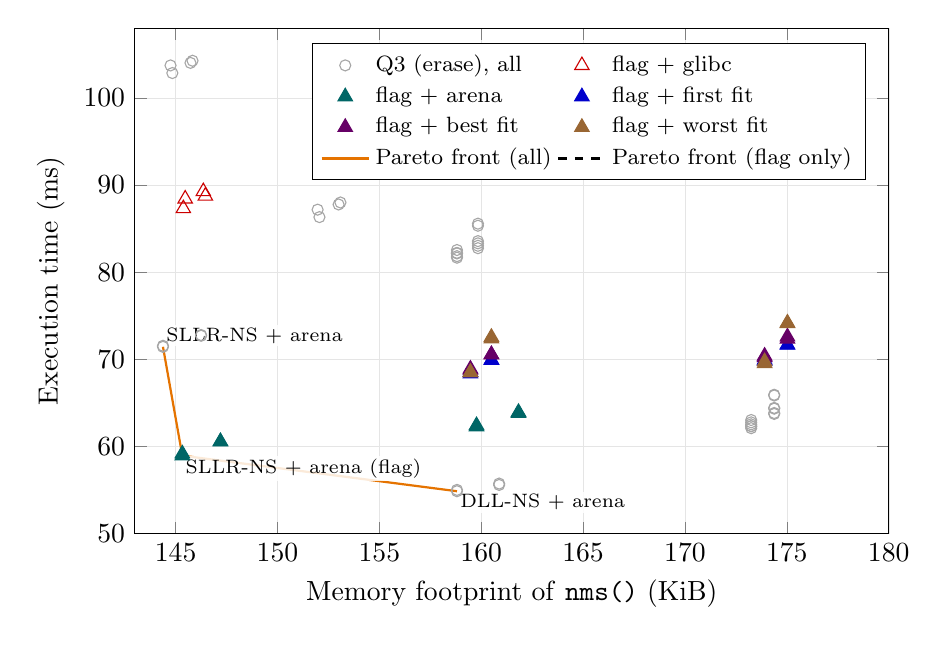
\begin{tikzpicture}
\begin{axis}[width=0.92\textwidth, height=8cm, grid=both, grid style={line width=.1pt, draw=gray!20}, legend cell align={left}, legend style={font=\footnotesize}, xlabel={Memory footprint of \texttt{nms()} (KiB)}, ylabel={Execution time (ms)}, legend pos=north east, xmin=143, xmax=180, ymin=50, ymax=108, legend columns=2]
\addplot[only marks, mark=o, mark size=2pt, color=gray!70] coordinates {(289.00,347.539) (289.05,357.276) (145.73,104.023) (153.00,87.773) (145.83,104.266) (153.09,88.000) (144.75,103.730) (151.97,87.177) (144.84,102.856) (152.06,86.323) (493.78,352.303) (288.69,351.790) (288.69,351.280) (288.69,352.251) (146.25,72.708) (159.84,82.756) (159.84,83.312) (159.84,85.334) (160.88,55.587) (174.38,63.737) (174.38,64.339) (174.38,65.849) (146.25,72.791) (159.84,83.032) (159.84,83.569) (159.84,85.572) (160.88,55.744) (174.38,63.842) (174.38,64.427) (174.38,65.935) (144.38,71.554) (158.81,81.666) (158.81,82.209) (158.81,81.843) (158.81,54.865) (173.25,62.340) (173.25,62.768) (173.25,62.102) (144.38,71.436) (158.81,82.160) (158.81,82.546) (158.81,82.198) (158.81,55.018) (173.25,62.541) (173.25,63.037) (173.25,62.321)};
\addlegendentry{Q3 (erase), all}
\addplot[only marks, mark=triangle, mark size=3pt, color=red!80!black] coordinates {(289.05,89.016) (146.36,89.268) (153.63,95.000) (146.46,88.751) (153.72,94.268) (145.38,87.310) (152.60,92.880) (145.47,88.421) (152.69,94.067)};
\addlegendentry{flag + glibc}
\addplot[only marks, mark=triangle*, mark size=3pt, color=teal!80!black] coordinates {(494.62,83.017) (147.20,60.575) (161.83,63.825) (147.20,60.539) (161.83,63.928) (145.33,59.171) (159.77,62.416) (145.33,58.947) (159.77,62.282)};
\addlegendentry{flag + arena}
\addplot[only marks, mark=triangle*, mark size=3pt, color=blue!80!black] coordinates {(288.69,82.780) (160.50,69.912) (175.03,71.649) (160.50,69.935) (175.03,71.680) (159.47,68.346) (173.91,69.816) (159.47,68.541) (173.91,69.940)};
\addlegendentry{flag + first fit}
\addplot[only marks, mark=triangle*, mark size=3pt, color=violet!80!black] coordinates {(288.69,82.514) (160.50,70.549) (175.03,72.598) (160.50,70.553) (175.03,72.350) (159.47,68.787) (173.91,70.233) (159.47,68.898) (173.91,70.383)};
\addlegendentry{flag + best fit}
\addplot[only marks, mark=triangle*, mark size=3pt, color=brown!80!black] coordinates {(288.69,83.257) (160.50,72.375) (175.03,74.114) (160.50,72.546) (175.03,74.184) (159.47,68.462) (173.91,69.535) (159.47,68.532) (173.91,69.749)};
\addlegendentry{flag + worst fit}
\addplot[thick, color=orange!90!black, mark=none] coordinates {(144.38,71.436) (145.33,58.947) (158.81,54.865)};
\addlegendentry{Pareto front (all)}
\addplot[thick, dashed, color=black, mark=none] coordinates {(145.33,58.947)};
\addlegendentry{Pareto front (flag only)}
\node[font=\scriptsize, anchor=south west, fill=white, fill opacity=0.85, text opacity=1, inner sep=1pt] at (axis cs:144.38,71.436) {SLLR-NS + arena};
\node[font=\scriptsize, anchor=north west, fill=white, fill opacity=0.85, text opacity=1, inner sep=1pt] at (axis cs:145.33,58.947) {SLLR-NS + arena (flag)};
\node[font=\scriptsize, anchor=north west, fill=white, fill opacity=0.85, text opacity=1, inner sep=1pt] at (axis cs:158.81,54.865) {DLL-NS + arena};
\end{axis}
\end{tikzpicture}
\caption{Μεγέθυνση στην περιοχή των λιστών, με τα Pareto optimal σημεία.}
\end{subfigure}
\caption{Pareto plot του Ζητουμένου 4: τα σημεία της εκδοχής με flags (τρίγωνα) και τα σημεία του Ζητουμένου 3 με erase (κύκλοι). Η συνεχής γραμμή είναι το Pareto front όλων των σημείων και η διακεκομμένη το Pareto front μόνο της εκδοχής με flags (εδώ ένα μόνο σημείο, SLLR-NS με arena).}
\label{fig:q4}
\end{figure}

\subsubsection*{Σχολιασμός Αποτελεσμάτων Ζητουμένου 4}
\textbf{Ο \en{vector} ωφελείται περισσότερο.} Χωρίς \en{\texttt{erase}} εξαφανίζονται οι μετακινήσεις των στοιχείων, και ο \en{vector} πέφτει από 357.28 σε 89.02 \en{ms} με \en{glibc} (4.0$\times$ γρηγορότερος), φτάνοντας τις λίστες με \en{glibc}. Η μνήμη του όμως μένει η ίδια (289 \en{KiB}, λόγω του διπλασιασμού της χωρητικότητας), οπότε δεν μπαίνει στο \en{Pareto front}.

\textbf{Η \en{SLL} γίνεται καλύτερη από τη \en{DLL}.} Στο Ζητούμενο 2 η \en{DLL} κέρδιζε γιατί η \en{\texttt{erase}} της \en{SLL} ψάχνει τον προηγούμενο κόμβο. Χωρίς \en{\texttt{erase}} αυτό το κόστος φεύγει: η \en{SLL} με \en{glibc} επιταχύνεται (104.0 $\rightarrow$ 89.3 \en{ms}), ενώ η \en{DLL} επιβραδύνεται (87.8 $\rightarrow$ 95.0 \en{ms}). Η επιβράδυνση οφείλεται στο ότι τα απορριφθέντα πλαίσια μένουν στη λίστα, οπότε κάθε επόμενο πέρασμα του εσωτερικού βρόχου τα διασχίζει ξανά (μαζί με τον έλεγχο του \en{flag}), ενώ με \en{erase} η λίστα μίκραινε. Τώρα η \en{SLL}, με μικρότερους κόμβους (160 έναντι 168 \en{B}, δηλαδή λιγότερα \en{bytes} ανά διάσχιση και καλύτερη χρήση της \en{cache}), είναι γρηγορότερη και μικρότερη από τη \en{DLL}, με όλους τους \en{allocators}.

\textbf{Μνήμη.} Το \en{vector} των \en{flags} προσθέτει ένα \en{byte} ανά πλαίσιο (μαζί με το \en{header} του \en{block}), δηλαδή μερικές εκατοντάδες \en{bytes} στο \en{peak} (π.χ. \en{SLL-NS} με \en{arena}: 147{,}840 $\rightarrow$ 148{,}816 \en{B}). Η δομή \en{\texttt{dets}} δεν μικραίνει πια, αλλά το \en{peak} της ήταν ούτως ή άλλως ολόκληρο το πιο φορτωμένο \en{frame}, πριν από οποιαδήποτε διαγραφή.

\textbf{\en{Fragmentation} (Πίνακας~\ref{tab:q4_frag}).} Επειδή όλα τα \en{blocks} μιας δομής έχουν το ίδιο μέγεθος και κάθε ελεύθερο \en{block} συγχωνεύεται με τους γείτονές του, οι \en{first/best/worst fit} δεν εμφανίζουν ουσιαστικό εξωτερικό κατακερματισμό: ένα ελεύθερο \en{block} χωρά πάντα τον επόμενο κόμβο. Ο κατακερματισμός είναι εσωτερικός, το \en{header} των 16 \en{B} και η στρογγυλοποίηση στα 16 \en{B} (7.5--8.9\% της μνήμης για τις λίστες), και, κυρίως, η αχρησιμοποίητη μνήμη του κομματιού του 1 \en{MiB} (83--84\% για τις λίστες). Ο \en{arena} δεν έχει \en{headers}, αλλά με τον \en{vector} «κατακερματίζει» με άλλο τρόπο: κρατά νεκρούς τους παλιούς \en{buffers} μέχρι το τέλος του \en{frame}.

\textbf{Ποια δομή και ποιος \en{allocator} είναι τώρα βέλτιστοι.} Στην εκδοχή με \en{flags} ο ταχύτερος συνδυασμός είναι \en{SLLR-NS} με \en{arena} (58.95 \en{ms}, 148{,}816 \en{B}), και το \en{Pareto front} της αποτελείται μόνο από αυτόν: είναι ταυτόχρονα ο ταχύτερος και (μαζί με \en{SLL-NS} με \en{arena}, ίδια μνήμη) ο μικρότερος. Το \en{Pareto front} όλων των σημείων (Σχήμα~\ref{fig:q4}) είναι: \en{SLLR-NS} με \en{arena} (\en{erase}) (147{,}840 \en{B}, 71.44 \en{ms}), \en{SLLR-NS} με \en{arena} (\en{flag}) (148{,}816 \en{B}, 58.95 \en{ms}), \en{DLL-NS} με \en{arena} (\en{erase}) (162{,}624 \en{B}, 54.87 \en{ms}).

\textbf{Άλλαξε η επιλογή σε σχέση με τα Ζητούμενα 2 και 3;} Ναι, ως προς τη δομή: στα Ζητούμενα 2 και 3 η γρηγορότερη ήταν η \en{DLL} (λόγω της φθηνής \en{\texttt{erase}}), ενώ με \en{flags}, όπου δεν υπάρχει \en{\texttt{erase}}, η απλούστερη και μικρότερη \en{SLL} είναι καλύτερη και στα δύο κριτήρια. Ο \en{allocator} δεν άλλαξε: ο \en{arena} παραμένει βέλτιστος, γιατί ο τρόπος που ζει η μνήμη (όλη ελευθερώνεται στο τέλος κάθε \en{frame}) δεν άλλαξε. Συνολικά, η αλλαγή στο πρόγραμμα άλλαξε τα \en{accesses} στη μνήμη και άρα το \en{Pareto front}: η \en{flag} εκδοχή προσθέτει στο \en{front} ένα σημείο με σχεδόν την ελάχιστη μνήμη και χρόνο μόλις 7\% πάνω από τον ελάχιστο, χωρίς όμως να ξεπερνά τον ταχύτερο συνδυασμό του Ζητουμένου 3.

% =============================================================================
\section{Συμπεράσματα}
% =============================================================================
\begin{itemize}
    \item Η αντικατάσταση του \en{\texttt{std::vector}} με συνδεδεμένη λίστα (\en{DDTR}) μείωσε τον χρόνο εκτέλεσης της \en{NMS} έως 4$\times$ και το \en{memory footprint} στο μισό, επειδή η \en{\texttt{erase}} γίνεται $O(1)$ και η λίστα δεν δεσμεύει περιττή χωρητικότητα.
    \item Ο \en{allocator} (\en{DMM}) έδωσε ακόμη 30--37\% στον χρόνο. Ο \en{arena allocator} ταιριάζει στον κύκλο ζωής των δεδομένων της \en{NMS} και είναι ο βέλτιστος σε κάθε ζητούμενο, εκτός από τον συνδυασμό του με \en{vector}.
    \item Η ταχύτερη λύση συνολικά είναι \en{DLL-NS} με \en{arena}, εκδοχή \en{erase} (54.87 \en{ms}, 162{,}624 \en{B}), 6.3$\times$ γρηγορότερη από την αρχική έκδοση. Με σχεδόν την ελάχιστη μνήμη (0.7\% πάνω από το ελάχιστο) και χρόνο μόλις 7\% μεγαλύτερο, η καλύτερη ισορροπία είναι \en{SLLR-NS} με \en{arena}, εκδοχή \en{flags} (58.95 \en{ms}, 148{,}816 \en{B}).
    \item Η βέλτιστη δομή εξαρτάται από τις λειτουργίες που κάνει το πρόγραμμα: με \en{\texttt{erase}} κερδίζει η \en{DLL}, με \en{flags} η \en{SLL}. Ο \en{roving pointer} δεν βοηθά όταν η διάσχιση γίνεται με \en{iterators}, ενώ η αφαίρεση του \en{sentinel} βοηθά λίγο σε μνήμη και χρόνο.
    \item Τα \en{LLC misses} (\en{\texttt{l2d\_cache\_refill}}) ήταν σχεδόν ίδια σε όλες τις εκδοχές, αφού τα δεδομένα ενός \en{frame} χωρούν στην \en{L2}, οι διαφορές στον χρόνο προέρχονται από τον αριθμό εντολών, τις μετακινήσεις δεδομένων και το κόστος των \en{\texttt{malloc}/\texttt{free}}.
\end{itemize}

\end{document}
